\section{ Physics Object Reconstruction} 
\label{sec:ParticleReconstruction}
Different particles leave unique signatures in different sub-detectors of ATLAS. Figure \ref{fig:ATLASTransverse} shows a schematic of a simplified representation of various particles passing through different sub-detectors and leaving various signatures. Physics object reconstruction is the process of interpreting these signals to meaningful information about the outgoing particles. This section discusses the detail of reconstruction relevant to the thesis. 

\begin{figure}[!htb]
    \centering
    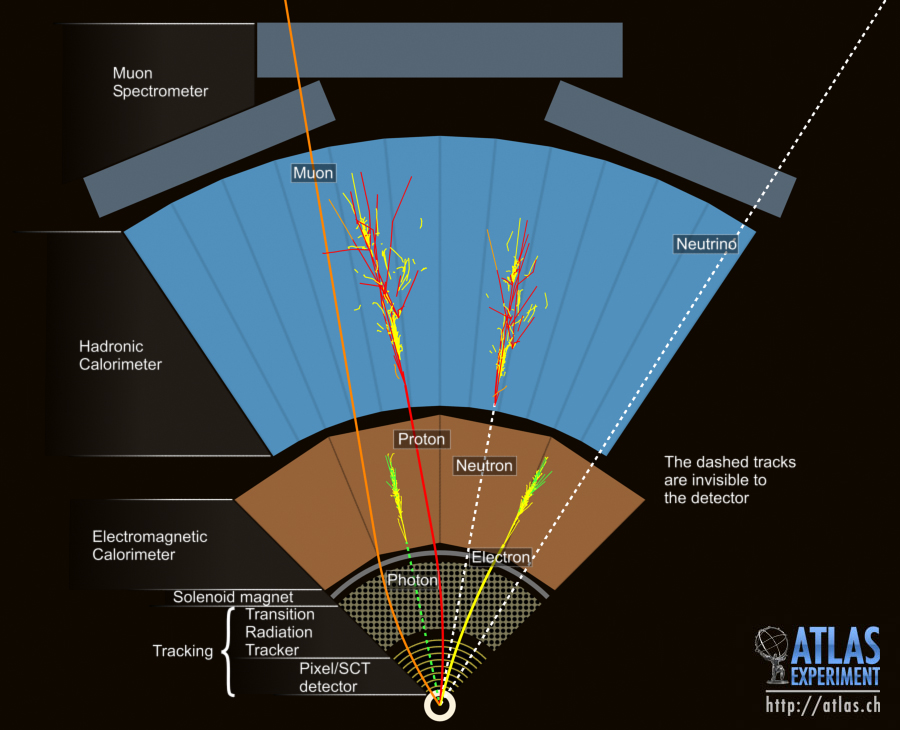
\includegraphics[width=.98\linewidth]{figures/LHC/ATLAS_Transverse.jpg}
    \caption{ Simplified representation of various particles traversing through different layers of ATLAS sub-detectors and leaving unique signatures \cite{ATLASTransverse}.\label{fig:ATLASTransverse}}
\end{figure}

\subsection{Trigger}
\label{subsec:TriggerATLAS}
The first step of particle and event reconstruction is selecting interesting high-energy events from a pool of lower-energy multiple-scattering signals. The high bunch crossing frequency of every $25$ ns results in a large amount of data making it physically impossible to store all events. ATLAS trigger system filters the events interesting for physics measurements to store permanently. 

ATLAS trigger consists of two levels, Level 1 (L1) trigger integrated into the hardware and high-level software trigger (HLT) \cite{TriggerSystemATLAS}. The L1 trigger is based on custom-built electronics, which uses signals from the calorimeters and muon trigger system (TGC and RPC) to identify event features such as electrons, photons, jets, taus, and missing energy. The L1 trigger reduces the $40$ MHz incoming collision data-rate corresponding to $25$ ns bunch crossing by a factor of $400$ to $100$ kHz output \cite{TriggerSystemATLAS}. The events accepted by the L1 trigger define regions of interest (ROI), and HLT algorithms are run on these events to select ones with candidate physics objects passing the kinematic requirements. The software-based HLT trigger further reduces the data rate by almost a factor of 100 to $1.5$ kHz \cite{ATLAS}. With the combination of L1 and HLT trigger system, the data rate is reduced by $400,000$, and the selected events corresponding to data readout of $1.5$ GB per second are stored in the permanent storage. Figure \ref{fig:DAQ} shows the schematic of ATLAS's trigger and data acquisition system. 

\begin{figure}[!htb]
    \centering
    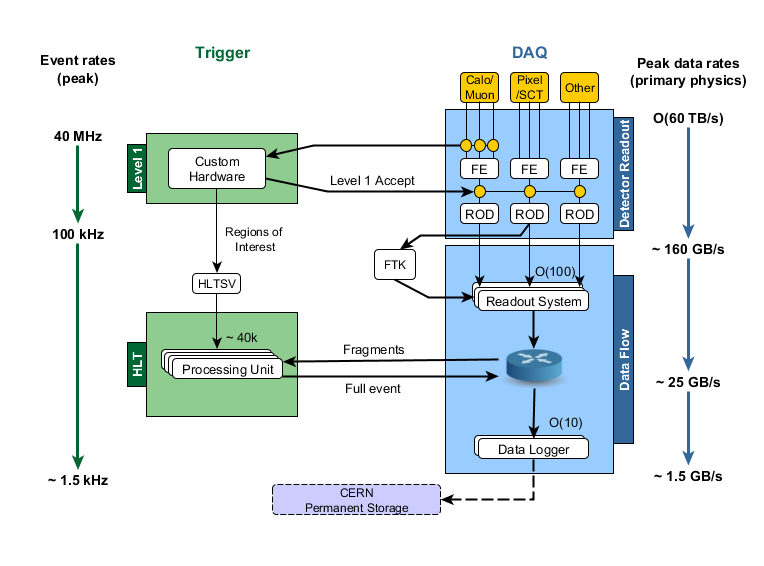
\includegraphics[width=.8\linewidth]{figures/LHC/DAQ_ATLAS.png}
    \caption{ Trigger and data acquisition system in ATLAS \cite{ATLAS_DAQ}.\label{fig:DAQ}}
\end{figure}

Physics object reconstruction discussed below converts the raw data output stored in permanent storage to physics objects used in physics analyses. 

\subsection{Tracks and Vertices Reconstruction}
\label{subsec:Tracking}
Tracking a charged particle is a critical step in reconstruction. The tracks of the charged particles play an essential role in momentum measurement, particle identification, and primary vertex reconstruction through the extrapolation of tracks to the interaction point. As the inner detector is closest to the beamline and comprises minimally ionizing detector material with high granularity, it plays a crucial role in track reconstruction. The ID magnetic field is homogenous, resulting in circular tracks of the charged particles. Five parameters shown in Figure \ref{fig:TrackParameter} define charged particle tracks; the ratio of charge and transverse momentum ($q/p_{T}$) defining the curvature; the distance of the closest approach to the primary vertex in $xy$-plane defining the transverse impact parameter ($d_{0}$), the longitudinal impact parameter ($z_{0}$) along the $z$-axis; the azimuthal angle ($\phi_{0}$) and the polar angle ($\theta_{0}$) of the particle direction at the closest approach point \cite{TrackingRun2_ATLAS}. 

\begin{figure}[!htb]
    \centering
    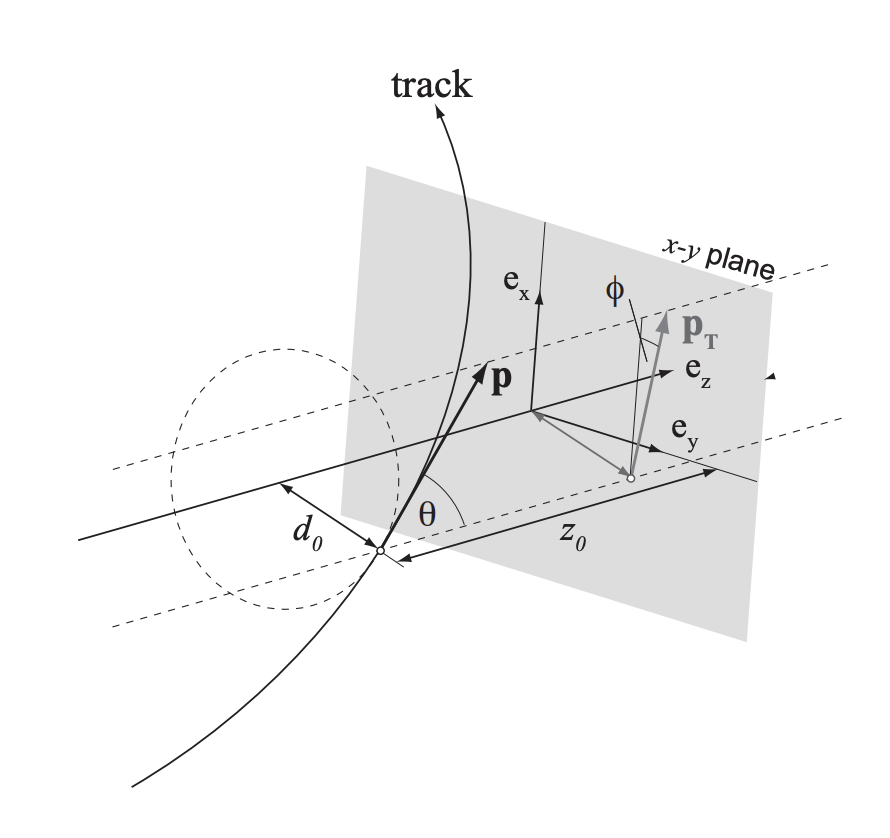
\includegraphics[width=.6\linewidth]{figures/LHC/TrackParameters.png}
    \caption{ Schematic showing the five-track parameters \cite{TrackParameterFig}.\label{fig:TrackParameter}}
\end{figure}

As shown by Figure \ref{fig:TrackingOutline}, track reconstruction used in Run-2 consists of two different approaches; the primary \textit{inside-out} approach and the secondary \textit{outside-in} approach \cite{TrackingRun2_ATLAS}. The first step in the inside-out track reconstruction is the space point and drift circle formation, formed respectively by the clusters of signals from the silicon detectors and drift-circles hits in the TRT. Second, track seeds are formed from a collection of three silicon-detector space points and extrapolated to the outer layers by including the compatible clusters in the track trajectory. Once the track is formed, an ambiguity resolution algorithm is applied to reassign shared clusters to the track with a better match, and the final track candidate is fitted using a global $\chi^{2}$ method. The last step of inside-out track reconstruction is adding compatible TRT drift holes and refitting the tracks. 

\begin{figure}[!htb]
    \centering
    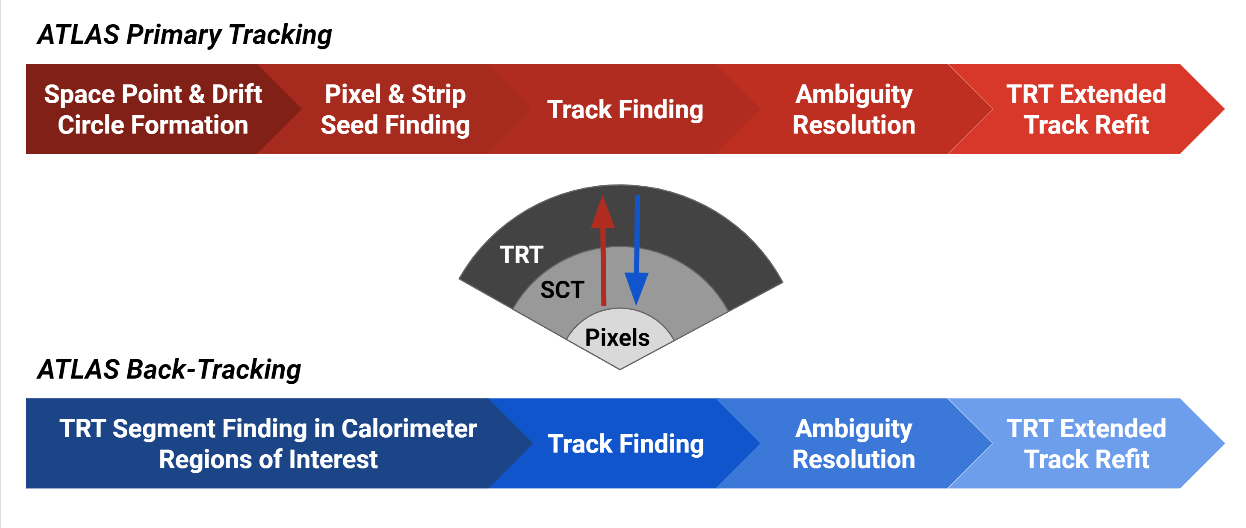
\includegraphics[width=.9\linewidth]{figures/LHC/trackingflowchart.png}
    \caption{Schematic showing the two techniques of track reconstruction, primary inside-out and secondary outside-in. The figure is taken from ATLAS Tracking CP group public tutorial \url{https://atlassoftwaredocs.web.cern.ch/trackingTutorial/idoverview/}. \label{fig:TrackingOutline}}
\end{figure}

The inside-out method is optimal for particles that minimally interact with the inner-detector material. However, secondary backtracking with an outside-in approach is needed for particles interacting with the inner detector, such as reconverted photons. In this approach, the track pattern recognition starts at the TRT in the regions of interest flagged by the electromagnetic calorimeter and backtracks to the silicon detectors. 

Tracks of the charged particle are extrapolated inward to the beamline and are assigned to vertices \cite{VertexReconstruction}. In most ATLAS analyses, including the one presented in this thesis, the space-point with the highest quadrature sum of track $p_T$ ($\sum_{track}{p_{T}^2}$) is identified as the primary vertex of an event.

\subsection{Electron Reconstruction}
\label{subsec:ParticleRecon_Elec}
Electrons, when interacting with a material, produce a photon by bremsstrahlung radiation, the process defining the interaction of a charged particle with the electric field of an atomic nucleus. Any energetic photon, either from a physics process or bremsstrahlung, can turn into a pair of $e^{+}e^{-}$, which can again radiate another set of photons, thus, giving rise to an electromagnetic shower. For given energy and material, electromagnetic showers have a characteristic penetration depth.

ATLAS electrons are reconstructed by combining the tracking information from the ID, and the energy deposits in nearby cells of the calorimeter,  energy clusters \cite{ElectronReco}. The clusters are formed only if the energy deposit exceeds four times the expected deposits from the pile-up. The reconstruction efficiency for high-energy electrons with transverse energy ($E_{T}>15$ GeV) is about $97-99\%$ \cite{ElectronReco}. \textit{Prompt electrons} originate from the hard scattering and are the primary interest of physics analysis. However, the detector has electrons from \textit{non-prompt sources} including the jets, misidentification, and pile-up. Therefore it is imperative to identify and isolate the prompt electrons in an event, and the efficiency for identification and isolation varies with its kinematic such as $\eta$ or $E_{T}$. Limited by the coverage of the electromagnetic calorimeter, only electrons within the $|\eta| <2.47$ range can be reconstructed and identified as prompt in ATLAS.

The electron identification is based on a multivariate-likelihood (LH) technique which takes information from tracking detectors and calorimeters as input. The tool is trained to separate signal and background probability density functions using simulated $Z \rightarrow e^{+}e^{-}$ and $J / \psi \rightarrow e^{+}e^{-}$ events. The LH tool provides four \textit{working points}, VeryLoose, Loose, Medium, and Tight, at different values of the LH discriminant to cover various needs of several ATLAS analyses. The analysis presented in this thesis uses electrons satisfying the Loose identification working point with at least one hit in the IBL. 

Prompt electrons originating from W, Z, or H decay are characterized by low activity around them in the $\eta-\phi$ plane. An isolation requirement is applied to the electron candidates to select ones from the hard scattering. Calorimeter and track-based requirements on isolation variables are defined to quantify the isolation. The variables are based on the amount of activity around an isolation cone of the candidate electron. Calorimeter-based isolation relies on the variable $E_{T,cone}^{iso}$, the sum of transverse energies inside a $\deltaR=0.2$ cone of the electron candidate. Similarly, the track-based isolation variable is $p_{T,cone}^{iso}$, the sum of the transverse momentum of the electron candidate within a $p_{T}-$dependent $\Delta R$, which is defined as, 

\begin{equation}
\Delta R = min \left( \frac{10 ~ GeV}{p_{T}},\Delta R_{max} \right)
\end{equation}
where the maximum cone size is $\Delta R_{max} = 0.2$. Similar to the identification, several working points are available for electron isolation. The measurement in this thesis uses the \textit{Loose$\_$VarRad} isolation working point which requires $E_{T,cone}^{iso} < 0.3$ and $p_{T,cone}^{iso} < 0.15$. Figure \ref{fig:ElecEff} shows the electron identification and isolation efficiencies as a function of their $E_{T}$. The Loose working point has the highest identification and isolation efficiencies and is the optimal working point for the measurement because of the fully reconstructable clean final state.

\begin{figure}[!htb]
    \centering
    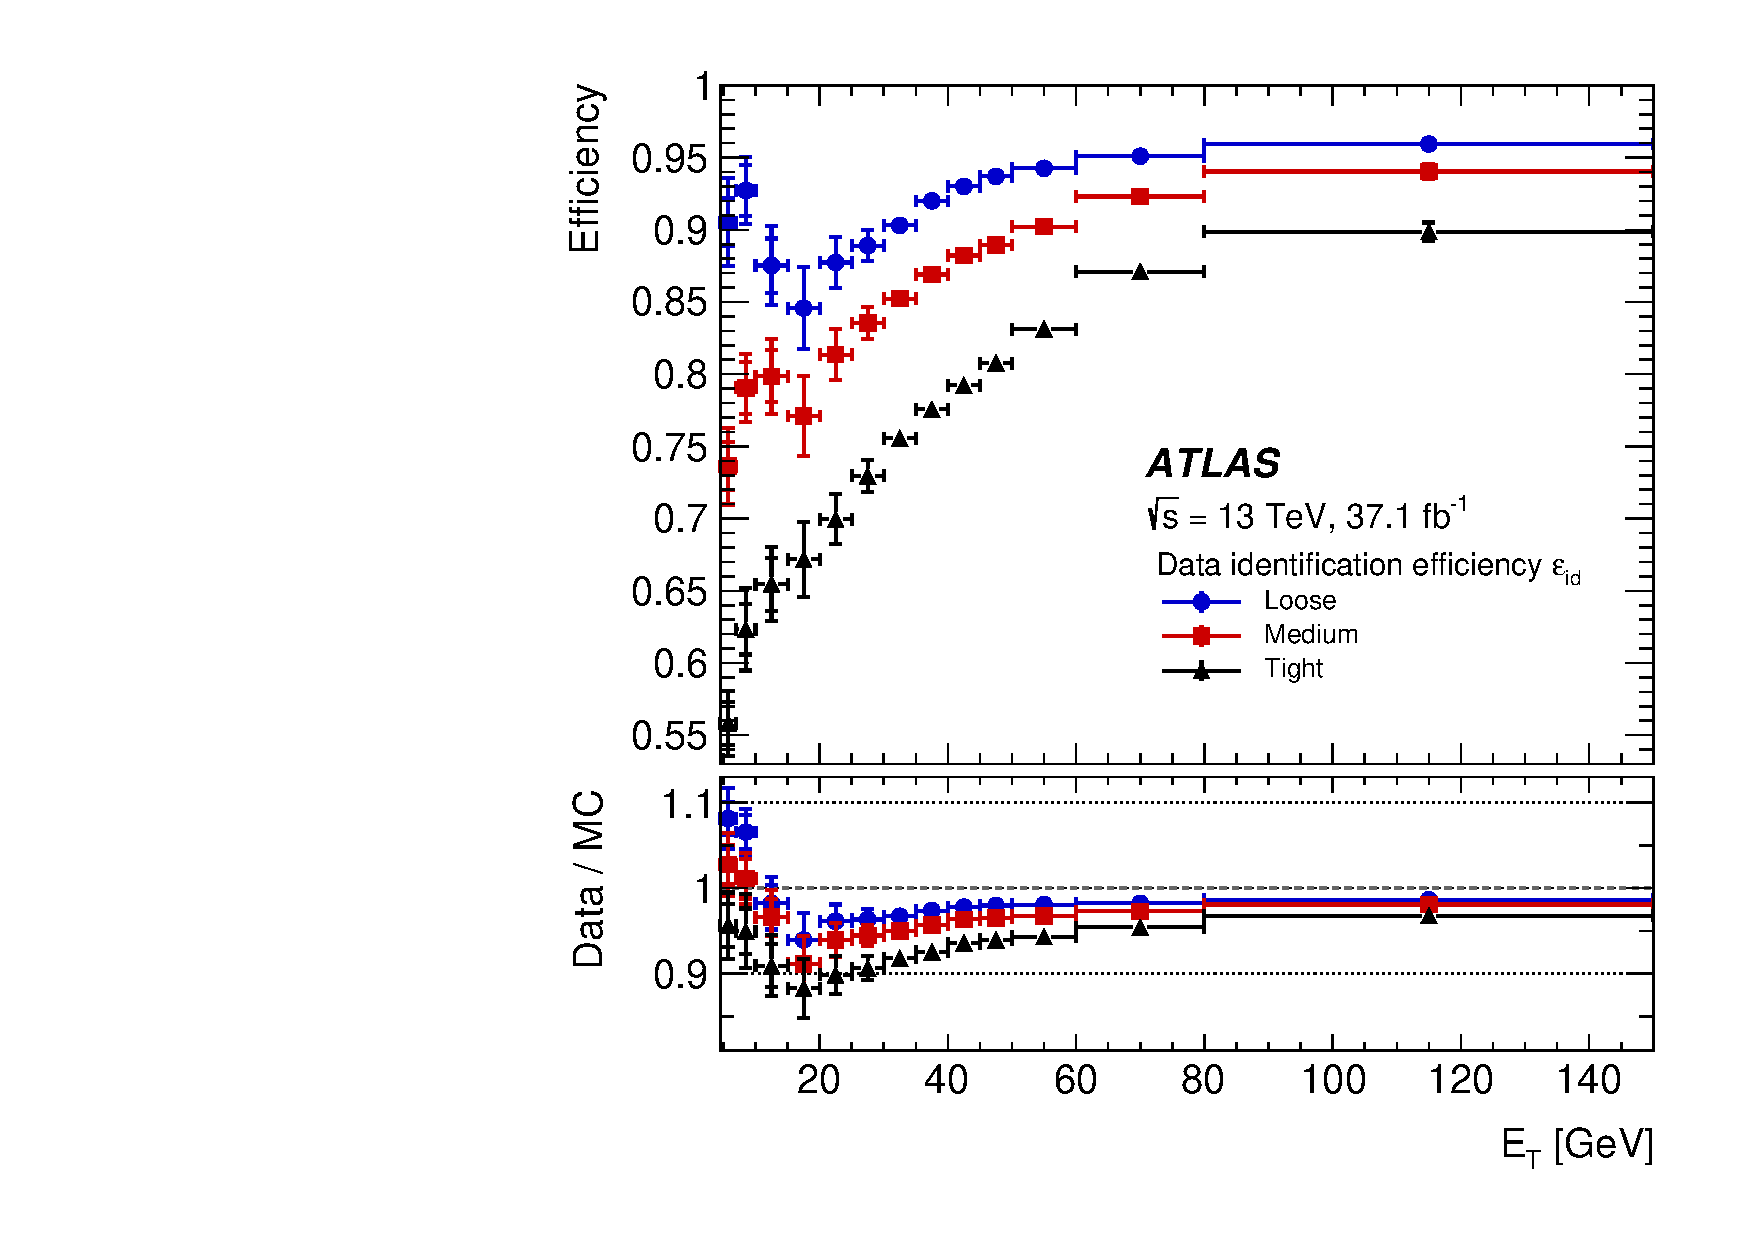
\includegraphics[width=.49\linewidth]{figures/LHC/ElecIdent_Eff.pdf}
    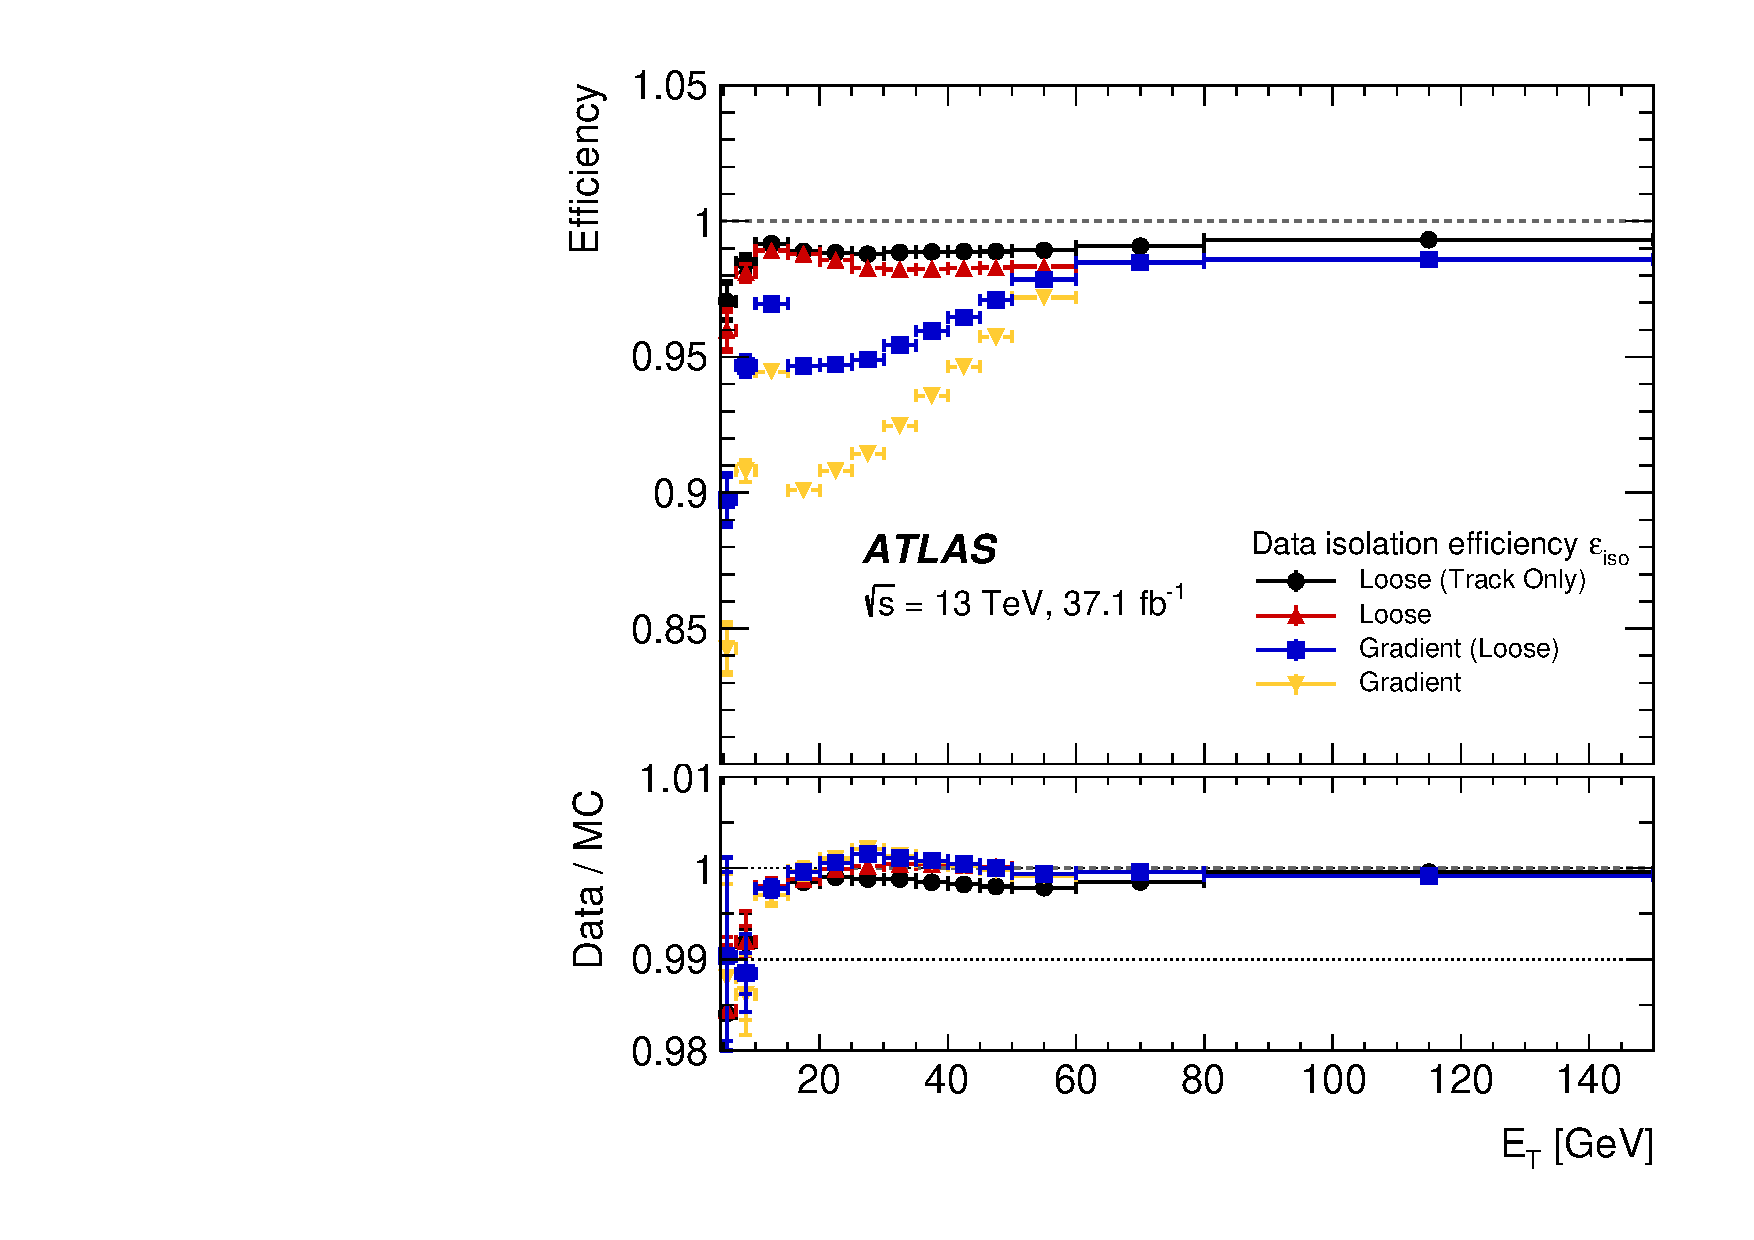
\includegraphics[width=.49\linewidth]{figures/LHC/Elec_IsoEff.pdf}
    \caption{ Distributions showing the identification (left) and isolation (right) efficiencies for electrons in data as a function of their $E_{T}$\cite{ElectronReco}.\label{fig:ElecEff}}
\end{figure}

The total electron efficiency is defined as the product of the electron reconstruction, identification, isolation, and trigger efficiencies as, 

\begin{equation}
    \epsilon_{total} = \epsilon_{reco} \times \epsilon_{id} \times \epsilon_{iso} \times \epsilon_{trigger}     
\end{equation}

Each of the efficiency terms is evaluated on data and MC. \textit{Scale Factors (SF)} defined as the ratio of the measured efficiency in data and the efficiency simulated in MC are derived and applied to the simulation to match the one observed in the data. Typically, SFs are close to one, and systematic uncertainties related to the electron reconstruction, identification, isolation, trigger efficiency, and the different scale factors are considered in the measurement.

\subsection{Muon Reconstruction}
\label{subsec:ParticleRecon_Muon}
The rate of bremsstrahlung radiation is inversely proportional to the square of a particle's mass. Since muons are about $200$ times heavier than electrons, they primarily interact with the detector material through ionization. Therefore, muons are minimally ionizing particles that do not create electromagnetic shower in the calorimeters and pass through all layers of the ATLAS detector. Hence, muon detection relies on track measurements from the inner detector and muon spectrometer. As shown in Figure \ref{fig:MuonFig}, four types of muons are defined based on the type of sub-detectors used during a muon reconstruction,

\begin{itemize}
    \item{\textbf{Combined muons:} muons reconstructed from a global refit of ID and MS tracks }
    \item{\textbf{Segment-tagged muons:} muons reconstructed from a fitted ID track and MS segment track } 
    \item{\textbf{Calo-tagged muons:}  muons reconstructed using ID track matched to the minimum ionizing energy deposits in the calorimeters}
    \item{\textbf{Standalone Muons:} muons reconstructed solely from the MS tracks }
\end{itemize}

\begin{figure}[!htb]
    \centering
    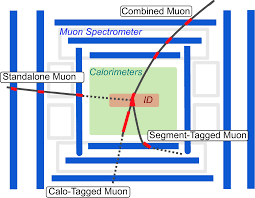
\includegraphics[width=0.7\linewidth]{figures/LHC/MuonTypes.png}
    \caption{ Schematic of four different types of muons reconstructed using several layers of sub-detectors \cite{MuonFig}.\label{fig:MuonFig}}
\end{figure}

Similar to the electron reconstruction discussed in Section \ref{subsec:ParticleRecon_Elec}, reconstructed muons from the hard scatter are identified and isolated from the muons originating from secondary sources. Muon identification working points are developed by applying quality requirements in the simulated $t\bar{t}$ events where a $W$ from top-quark decays to a muon and a neutrino. The quality cuts require at least one-pixel hit, five SCT hits, and not more than three pixel or SCT holes. At least $10\%$ of TRT hits are included in the fit for the $0.1<\eta<0.9$ range with full TRT coverage \cite{MuonReco}. Three variables are used in muon identification; $q/p$ significance, which is defined as the ratio of muon's charge and momentum divided by the sum-quadrature of their uncertainties; $\rho^{'}$ defined as the absolute difference of transverse momentum measurements in the ID and MS divided by the combined track's $p_{T}$; and the normalized $\chi ^{2}$ of the combined track fit \cite{MuonReco}. 
Four identification \textit{working points}, Loose, Medium, Tight, and High-$p_{T}$ are defined for muons in Run-2. The measurement uses a Loose identification point, which comprises all four types of muons and is developed specifically for processes with four leptons in the final state  \cite{MuonReco}. 

To evaluate the total reconstruction efficiency of muons, $Z \rightarrow \mu^{+}\mu^{-}$ and $J/\psi \rightarrow \mu^{+}\mu^{-}$ events are used. The reconstruction efficiency in the region with ID coverage $|\eta|<2.5$ is obtained by using the tag-and-probe method, whereas, for $|\eta|>2.5$ region, it is estimated by evaluating SFs based on a double ratio of data and MC in $Z \rightarrow \mu\mu$ events \cite{MuonEffLargeEta}.

Analogous to electrons, muons are required to meet calo-based and ID-based isolation requirements. Muons in the measurement satisfy \textit{PflowLoose$\_$VarRad} isolation working point. Like in the case of electrons, the total efficiency for muon reconstruction and selection is the product of reconstruction, identification, isolation, and trigger efficiencies. The systematic uncertainties on each part of electron reconstruction and different scale factors are propagated to the final cross-section measurement.

\subsection{Jet Reconstruction}
\label{subsec:ParticleRecon_Jets}

Due to color confinement in QCD, a quark or gluon cannot exist on its own and goes through hadronization to form a collimated color-neutral stream of particles, \textit{jets}. Generally, jets are deeply penetrating, passing through the electromagnetic calorimeter, and gets fully absorbed by the material in the hadronic calorimeter. ATLAS jet reconstruction relies on the formation of \textit{topo-clusters}, energy deposits in the calorimeter cells using a sequential recombination algorithm. Most commonly, the jets are reconstructed using a type of sequential algorithm, the anti-$k_{T}$ algorithm. At first, pseudojets are formed by iteratively combining nearby particles based on a specific metric distance to other particles from the pseudojet. The iteration is continued over a set of nearby particles until the pseudojets' metric distance is smaller than that between the pseudojet and the nearby particle. For the anti-$k_{T}$ algorithm, the separation distance metric is based on their transverse momenta \cite{AntiKtAlgo}. A radius parameter for jets determines the angular size of resulting jets in the $y-\phi$ plane. 

The analysis reported here uses jets reconstructed using the anti-$k_{T}$ algorithm with a particle flow implementation \cite{ParticleFlow}\cite{AntiKtAlgo}. The particle flow reconstruction technique was first implemented by ATLAS reconstruction in Run$-2$. It combines information from the inner detector tracks and the calorimeter's topo-clusters. It has advantages over simple cluster-based algorithms because the tracking detector has a better momentum resolution for lower-energy charged particles, extending the reconstruction to include particles with topo-cluster energy deposits lower than the noise thresholds \cite{ParticleFlow}. The particle flow algorithm removes cluster contributions from pile-up using track-to-vertex association. Figure \ref{fig:PflowJets} shows a schematic of the particle flow jet reconstruction algorithm used in ATLAS.

\begin{figure}[!htb]
    \centering
    
\includegraphics[width=0.99\linewidth]{figures/LHC/fig_02.png}
    \caption{ Schematic of particle flow jet reconstruction \cite{ParticleFlow}.\label{fig:PflowJets}}
\end{figure}

First, ID tracks and topo clusters are reconstructed. If an ID track matches the topo-cluster, the tracks are used for jet reconstruction, and the cluster is modified by subtracting the energy of the used tracks. In the case of neutral jets or jets outside the geometrical acceptance of ID, only the topo-clusters are used as input for jet reconstruction. Figure \ref{fig:PflowvsCalo} shows the improvement in jet transverse momenta resolution when using the particle flow algorithm over the cluster-based algorithm as a function of jet's $p_{T}$ (left) and $\eta$ (right). The distributions show the resolution is improved significantly for low$-p_{T}$ and central jets having low $\eta$ with particle flow algorithm.

\begin{figure}[!htb]
    \centering
    \includegraphics[width=.48\linewidth]{figures/LHC/Pflow_vs_Calo_pt.pdf}
    \includegraphics[width=.48\linewidth]{figures/LHC/Pflow_vs_Calo_eta.pdf}
    \caption{ Resolution of jet transverse momentum for only cluster-based jets (LC+JES) and particle flow jets as a function of $p_{T}$ (left) and $\eta$ (right) \cite{ParticleFlow}.\label{fig:PflowvsCalo}}
\end{figure}

Jet energies are highly susceptible to pile-up density, and jets constitute various particles that could interact differently with various sub-detectors. Therefore, the reconstructed jets must be calibrated before being used in the measurement. Figure \ref{fig:JetCalib} schematically shows different steps of jet calibration, which is discussed in detail in Ref \cite{JetCalib}. The first step in jet calibration is an event-by-event subtraction of pile-up-related average energy density ($\rho$) from jet candidate energy. The pile-up is first corrected as a function of $p_{T}$, then as a function of average pile-up density ($\mu$) and the number of primary vertex per event ($N_{PV}$). The second set of jet calibration accounts for the detector response, correcting for the interaction with the detector's passive material and possible flavor dependence on the detector response. \textit{In-situ} calibration is the final part of the jet calibration, which accounts for the differences in jet response measured in data and MC. 

\begin{figure}[!htb]
    \centering
    \includegraphics[width=.95\linewidth]{figures/LHC/JetCalib.pdf}
    \caption{ A schematic of different steps of jet calibration \cite{JetCalib}.\label{fig:JetCalib}}
\end{figure}

The analysis uses a \textit{Jet Vertex Tagger} (JVT) variable to differentiate hard-scattering jets from pile-up \cite{JVT}. The JVT variable is a multivariate combination of two variables; first, the \textit{jet-veretex-fraction} defined as a fraction of the total momentum of tracks in jet associated with the primary vertex, and second, the number of reconstructed primary vertices in an event ($N_{PV}$) \cite{JVT}. To identify the jets from hard scattering outside the ID acceptance in $2.5<|\eta|<4.5$ range, a \textit{forward Jet Vertex Tagger} (fJVT) discriminant is used, which is derived by exploiting the topological correlations among particles from a pile-up interaction \cite{fJVT}. 

The systematic uncertainties related to each step of jet reconstruction, calibration, and JVT/fJVT tagging are propagated to the final measurements of the unfolded differential cross-sections.  
